\section{Our Contributions}\label{sec:Contributions}

We will present the SHE problem as an optimal control one, where the optimization variable is the signal $u(\tau)$ defined in the entire interval $[0,\pi)$. 
%
In particular, we will describe how the Fourier coefficients of the function $u(\tau)$ can be seen as the final state of a system controlled by $u (\tau)$, and where the control must be a piece-wise constant function. In order to simplify the reading, we will define this type of controls as:

\vspace{1em}
\begin{definition}[Digital control of $\mathcal{U}$]
    A control $u(\tau)$ is called digital if, for each time $\tau\geq 0$, it only takes values in the finite set of real number $\mathcal{U}$ except a finite set of values (switching angles).  
\end{definition}
%
%Hence, the optimization is performed among all the possible functions that satisfy $|u(\tau)|<1 $ and can control the final state at the desired Fourier coefficients. 
%
%Then we will show how to design a control problem so that the solution is a digital control of $\mathcal{U}$.
%
%%%%%%%%%%%%%%%%%%%%%%%%%%%%%%%%%%%
%
%In this formulation, the SHE problem converts in a minimization problem with restrictions which can be solved by well-known techniques. 
%
%Since the problem has several minimizers, we shall solve it employing global optimizers. 
%
%Furthermore, since the choice of the waveform is arbitrary, we shall proceed in the same way for each possible waveform. 
%
We briefly mention our contributions below, ad then explain each of them in detail:
\begin{enumerate}
    \item Re-formulation of Problem \ref{pb:SHEp} as a control problem.
    \item Formulate a optimal control problem with penalization term order to obtain as solution a piece-wise  function which must be take only two posible values ($\mathcal{U} \in \{-1,1\}$)(\emph{bang-bang controls}).
    \item Formulate a optimal control problem with penalization term order to obtain as solution a piece-wise function.
    \item Describe a sufficients conditions of some penalization in optimal control problem to obtain a constant piece-wise function as solution
\end{enumerate}

\subsection{Reformulation of SHE problem as optimal control problem}

Taking into account that we have all the elements considered in the definition of the Problem \ref{pb:SHEp}, we introduce the following dynamic system:
\begin{equation}\label{eq:CauchyReversed}
    \begin{cases}
        \displaystyle\dot{\bm{x}}(\tau) = -\frac 2\pi\bm{\mathcal{D}}(\tau)u(\tau),  & \tau \in [0,\pi)
        \\[6pt]
        \bm{x}(0) = \bm{x}_0
    \end{cases},
\end{equation}
Where $\bm{x}(t) \in \mathbb{R}^{N_a + N_b}$ and $\bm{\mathcal{D}}(\tau) \in  \mathbb{R}^{N_a + N_b}$ is:
\begin{align*}
	\bm{\mathcal{D}}(\tau) = \begin{bmatrix} \bm{\mathcal{D}}^\alpha(\tau) \\ \bm{\mathcal{D}}^\beta(\tau) \end{bmatrix}     
\end{align*}
and where $\bm{\mathcal{D}}^\beta(\tau) \in \mathbb{R}^{N_a} $ and $ \bm{\mathcal{D}}^\beta(\tau) \in \mathbb{R}^{N_b}$ are,
\begin{gather}\label{eq:DalphaDbeta}
    \begin{align}
        \bm{\mathcal{D}}^\alpha(\tau) = 
        \begin{bmatrix} 
            \cos(e_a^1\tau) \\ \cos(e_a^2\tau) \\ \vdots \\ \cos(e_a^{N_a}\tau) 
        \end{bmatrix},
        \quad \bm{\mathcal{D}}^\beta(\tau) = 
        \begin{bmatrix} 
            \sin(e_b^1\tau) \\ \sin(e_b^2\tau) \\ \vdots \\ \sin(e_b^{N_b}\tau) 
        \end{bmatrix} 
    \end{align} 
\end{gather}
with set $\mathcal{E}_a$ and  $\mathcal{E}_b$ are:
\begin{align*}
	\mathcal{E}_a = \{e_a^1,e_a^2,e_a^3,\dots,e_a^{N_a}\}, \quad \mathcal{E}_b = \{e_b^1,e_b^2,e_b^3,\dots,e_b^{N_b}\}    
\end{align*}
%
Let this system, we can consider the following control problem:
\vspace{1em}
\begin{problem}\label{pb:SHEpControl}
    Let $\mathcal{U}$ be defined as in \eqref{eq:Udef} and let $\mathcal{E} _a $ and $\mathcal{E} _b $ be two sets of odd numbers with cardinalities $|\mathcal{E}_a| = N_a $ and $ |\mathcal{E} _b| = N_b$, respectively. Given the vectors $\bm{a}_T \in \mathbb{R}^{N_a}$ and $\bm{b}_T \in \mathbb{R}^{N_b} $, let us define $\bm{x}_0=[\bm{a}_T,\bm{b}_T]^\top \in \mathbb{R}^{N_a}\times\mathbb{R}^{N_b}$. We look for $u:\in [0,\pi)\to\mathcal{U}$ such that the solution of \eqref{eq:CauchyReversed} with initial datum $\bm{x}(0)=\bm{x}_0$ satisfies $\bm{x}(\pi)=0$.
\end{problem}
And given this control problem, we can formalate the following theorem:
\vspace{1em}
\begin{theorem}\label{th:SHEasDyn}
    The optimal control $u(\tau)$, the solution of Problem \ref{pb:SHEpControl}, is the piece-wise constante function that solve the Problem \ref{pb:SHEp}.
\end{theorem}

The Theorem \ref{th:SHEasDyn} is a directly consecuence of fundamental theorem of calculus. We have consider the formula integral of Fourier coefficients in its diferential form. In this way, the intragration from $\tau = 0$ to $\tau = \pi$ can be seen as a evolution of a dinamical system \eqref{eq:CauchyReversed} in the time interval $[0,\pi]$.

\begin{figure}[ht!] 
    \centering
    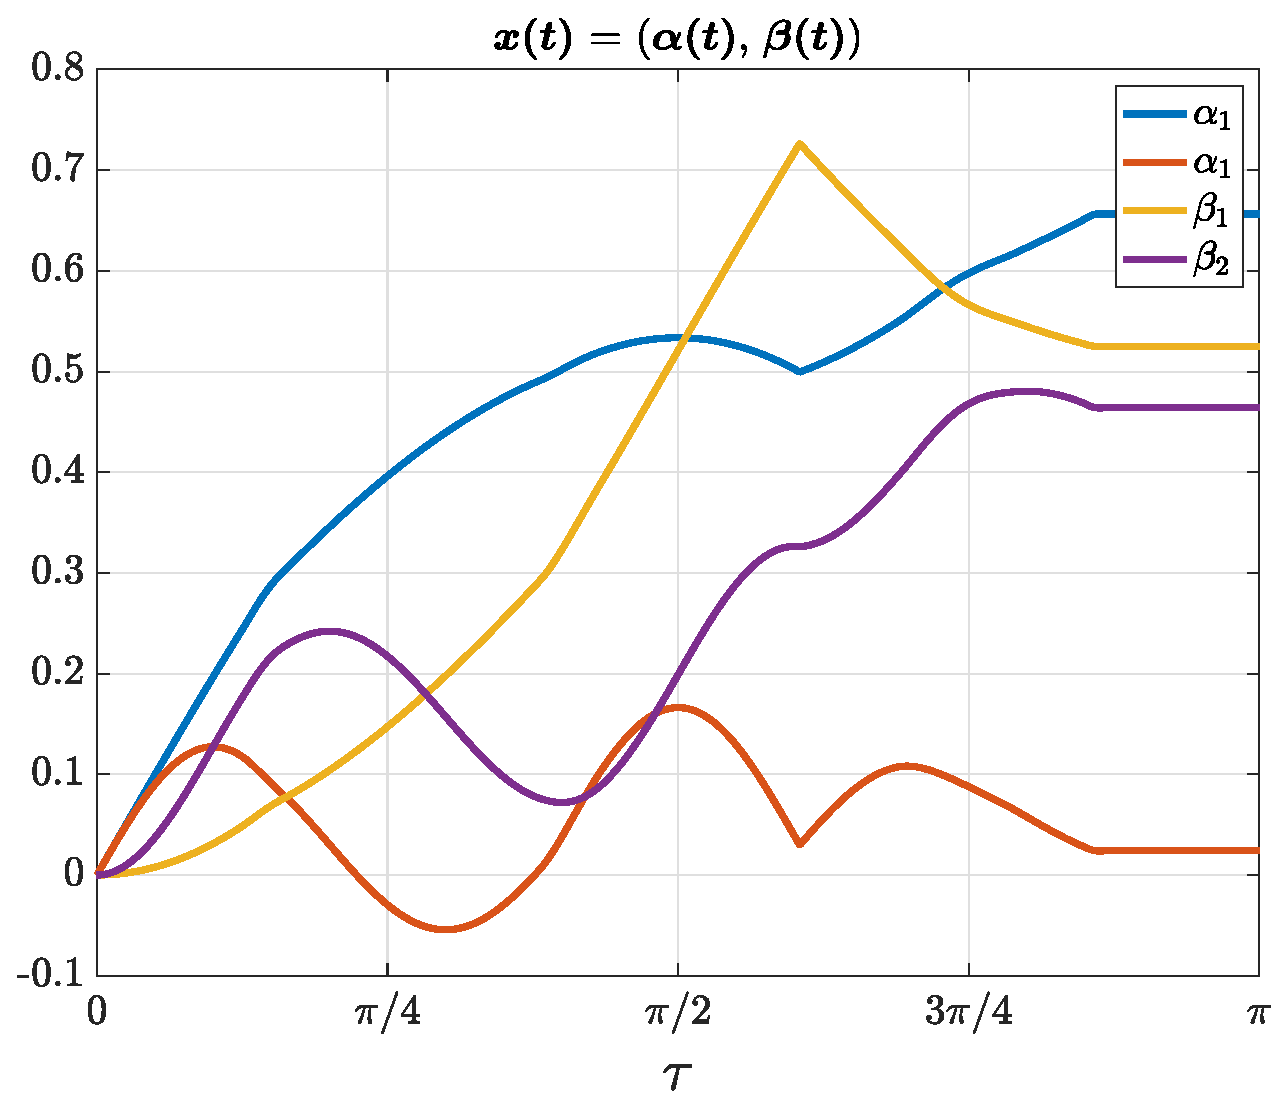
\includegraphics[scale=0.325]{img/fig02.eps}
    \caption{Evolution of ddinamical system \eqref{eq:CauchyReversed}$\mathcal{E}_a = \{1,2\}$ y $\mathcal{E}_b = \{1,2\}$ considerando el control $u(\tau)$ presentado en la Figura \ref{fig:exampleSHE}. Además mostramos las posiciones de los ángulos de conmutación $\bm{\phi}$.}
\end{figure}

Thank to this result, we can formulate a optimal control problem associated to the problem \ref{pb:SHEpControl}.

In what follows, for a given vector $\bm{v}\in\mathbb{R}^d$, we shall always denote by $\|\bm{v}\|$ the euclidean norm $\|\bm{v}\|_{\mathbb{R}^d}$.
\newline


\begin{problem}[OCP for SHE]\label{pb:OCP1}
Let $\mathcal U$ be defined as in \eqref{eq:Udef}. Given two sets of odd numbers $\mathcal {E}_a $ and $\mathcal {E}_b $ with cardinality $N_a$ and $N_b$, respectively, and given initial condition $\bm{x}_0\in \mathbb{R}^{N_a+N_b}$, we look for the function $u(\tau):[0,\pi)\to \mathcal U$ solution of the optimal control problem  
\begin{align*}
	&\min_{u \in \mathcal{U}}\;\frac 12 \|\bm{x}(\pi)\|^2
	\\
    &\notag \text{subject to: }\quad \begin{cases}
            \displaystyle \dot{\bm{x}}(\tau) = -\frac 2\pi\bm{\mathcal{D}}(\tau) u(\tau),  & \tau \in [0,\pi)\\[6pt]
            \bm{x}(0) = \bm{x}_0
    \end{cases}
    \end{align*}
\end{problem}
The solution of Problem \ref{pb:OCP1} may be quite complex to be obtained, due to the restriction on the admissible control values. 

In order to bypass this difficulty, following a standard optimal control approach, we can formulate an equivalent minimization problem in which, instead of looking for $u\in\mathcal U$, we simply require that $|u|<1$ and we introduce a penalization term to ensure that $u$ is digital control of $\mathcal{U}$.


%
This alternative optimal control problem, which can be solved more easily by employing standard tools, reads as follows:
\newline
\begin{problem}[Penalized OCP for SHE]\label{pb:OCP_penalizado}
Fix $\epsilon>0$. Given two sets of odd numbers $\mathcal E_a $ and $\mathcal E_b $ and the target $\bm{x}_T \in \mathbb {R}^{N_a + N_b}$, we look a digital control of $\mathcal{U}$ as the solution of:
\begin{align*}
	&\min_{|u|<1} \Bigg[\frac 12 \|\bm{x}(\pi) \|^2+ \epsilon \int_0^{\pi} \mathcal{L}(u(\tau)) d\tau \Bigg]  
\end{align*}
under the dynamics given by \eqref{eq:CauchyReversed}.
\end{problem}

In Problem \ref{pb:OCP_penalizado}, the penalization function $\mathcal L: \mathbb{R} \rightarrow \mathbb{R}$ will be chosen such that the optimal control $u^*$ is a digital control of $\mathcal{U}$. Furthermore, the parameter $\epsilon$ should be small so that the solution minimizes the distance from the final state and the target.

In general, a penalization function that gives us a digital control of $ \mathcal {U} $ is not obvious to achieve. If we consider the optimality conditions of the system \eqref{eq:CauchyReversed} (Pontryagin's minimum principle) we can obtain a function $ \mathcal{H}_m (u) $ (the Hamiltonian function) that characterizes the behavior of the solution of the Problem \ref{pb:numOCP2}.

\vspace{1em}
\begin{definition}[Hamiltonian]\label{def:Hamiltonian}
    Let a Problem \ref{pb:OCP_penalizado}, we define a function $\mathcal{H}_m:[-1,1]\rightarrow \mathbb{R}$ such that:
    \begin{gather}\label{Hm}
        \mathcal{H}_m(u) = \epsilon \mathcal{L}(u) - mu  |  \forall m \in \mathbb{R}
    \end{gather}
\end{definition}

Already defined the Hamiltonian function we can say that:

\vspace{1em}
\begin{proposition}\label{prop:Hamiltoniano}
    Let the Problem \ref{pb:OCP_penalizado} and his Hamiltonian function $\mathcal{H}_m$. If for all $m \in \mathbb{R} - \mathcal{M}$ all minimuns are in $\mathcal{U}$, so the solution of the Problem \ref{pb:OCP_penalizado} is a digital control of $\mathcal{U}$. Where $\mathcal{M}$ can be the empty set or a finite set of real values.  
\end{proposition}

Thanks to the Proposition \ref{prop:Hamiltoniano}, we can design the penalization functions such that the Hamiltonian $\mathcal{H}_m$ only have minimuns in $\mathcal{U}$.

\subsection{SHE bi-nivel via OCP (Bang-Bang Control)} 

Now, we consider the case which the set of admisible controls is  $\mathcal{U}=\{-1,1\}$. The reader can note that this type of solutions in control theory literature is named \emph{bang-bang control}, while in Selective Harmonic Elimination literature is named bi-level solutions.
\vspace{1em}
\begin{theorem}\label{th:bang-bang}
    Let the Problem \ref{pb:OCP_penalizado} with the admisible control set  $ \ \mathcal{U} = \{-1,1\}$. If the function $\mathcal{L}$ is concave in the interval $[-1,1]$, so the optimal control is a digital control of $\mathcal{U} =  \{-1,1\}$.
\end{theorem}

Si aceptamos la Proposición \ref{th:bang-bang} es evidente que  para obtener un control digital de $\mathcal{U}=\{-1,1\}$ los mímimos Hamiltoniano $\mathcal{H}_m$ para todo $m\in \mathbb{R}-\mathcal{M}$ deben encontrarse en los bordes del intervalo $[-1,1]$ de manera que es suficiente considerar una función concava en el interior de este intervalo. 

Ilustramos esta idea en la Figura \ref{fig:Bang-Bang-penalization}, de manera que en la primera columna presentamos tres funciones de penalización compatible con la Proposición \ref{th:bang-bang} ($\mathcal{L}(u) = u$, $\mathcal{L}(u) = -u$, $\mathcal{L}(u) = -u^2$ ). Además mostramos a la derecha de cada una de ellas mostramos el comportamiento del Hamiltoniano para distintos valores de $m$ en diferentes colores y para cada una de ellas marcamos el mímimo del mismo color. Podemos ver que los mínimos en cada caso siempre siempre esta en $\mathcal{U}= \{-1,1\}$.
\begin{figure} 
    \centering
    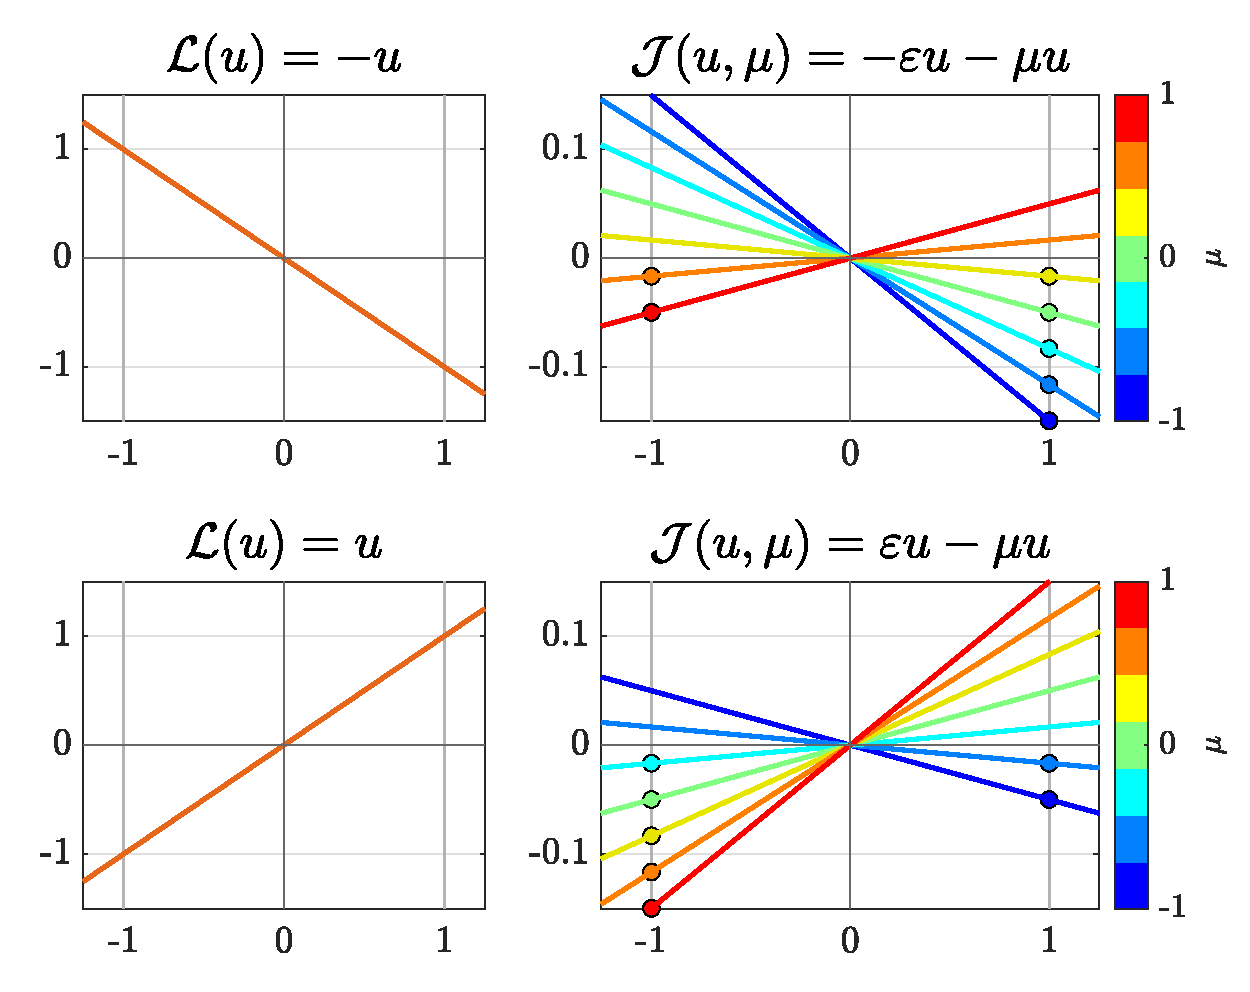
\includegraphics[scale=0.415]{img/fig03.eps}
    \caption{SHE bi-level.} \footnotesize En la primera columna mostramos tres tipos de penalización concavas compatibles con la Proposición \ref{th:bang-bang}. A la derecha de cada una de ellas mostramos el comportamiento del Hamiltoniano para cada distintos valores de $m$ (colores). 
    \footnotesize

    \label{fig:Bang-Bang-penalization}
\end{figure}
\subsection{SHE multi-nivel via Piecewise linear penalization}

Gracias al caso bi-nivel podemos notar que si definimos una función de penalización $\mathcal{L}$ que entre dos valores $u_1$ y $u_2$ no tenga mímimos, es decir sea concava entre esos dos puntos entonces la función Hamiltoniana no tendrá el mímimos en $u \in (u_1,u_2)$ más que para un valor de concreto de $m$. Gracias a esta observación podemos afirmar que:

\vspace{1em}
\begin{theorem}\label{th:PLP}
    Given a set $\mathcal{U}$, we can choose the affine interpolation of a parabola $\mathcal{L}^{p_!}:[-1,1] \rightarrow \mathbb{R}$ as a penalization term. That is
    \begin{gather}\label{eq:PLP}
        \mathcal{L}^{p_1}(u) = \begin{cases}
            \lambda_k^{p_1}(u) & \text{if }  u \in [u_k,u_{k+1}[ \\
            1 & \text{if } u = u_{N_u} 
        \end{cases} \\
        \notag \forall k \in \{1,\dots,N_u-1\} 
    \end{gather}
    Donde 
    \begin{gather}
        \lambda_k^{p_1}(u) = (u_{k+1}+u_{k}) (u-u_k) + u_k^2
    \end{gather}
    De modo que el problema de \ref{pb:OCP_penalizado} con la penalización $\mathcal{L}(u)$ presentada antes tiene como solución un control digital del conjunto $\mathcal{U}$.
\end{theorem}
\vspace{1em}
\begin{remark}[\emph{Bang-off-bang}]
    En este caso, podemos notar que cuando consideramos un conjunto de controles admisibles como $\mathcal{U}= \{-1,0,1\}$ recuperamos la penalización de norma $L^1$. Este tipo de penalización añadido a la restricción $|u|<1$ nos da controles \emph{bang-off-bang}, bien conocidos en la literatura de control \cite{Wang2020}
\end{remark}

De la misma forma que en caso anterior en la Figura \ref{fig:SHE-multi} ilustramos como la penalización \eqref{eq:PLP} logra cumplir las condiciones de la proposición \ref{prop:Hamiltoniano}. Y por tanto esta penalización da lugar a una control óptimo digital de $\mathcal{U}$. 


\subsection{General conditions for  SHE multi-nivel}   

Como podemos observar el caso anterior no es más que una caso concrerto de condiciones más generales. De manera que podemos afirmar que: 
\vspace{1em}
\begin{theorem}\label{th:GeneralP}
    Assume that the finite set $\mathcal{U}$ defined in \eqref{eq:Udef} is composed by elements in ascending order. Let $\mathcal{Y} = \{y_\ell\}_{\ell=1}^L$ be another finite set, with the same cardinality as $\mathcal U$, such that the $L-1$ tuple
    \begin{gather}
        \frac{\Delta \mathcal{Y}}{\Delta \mathcal{U}} = \Bigg( \frac{y_\ell - y_{\ell+1}}{u_\ell - u_{\ell+1}} \Bigg)_{\ell=1}^{L-1}
    \end{gather}  is monotone. Let $\mathcal{L}:\mathbb{R} \rightarrow \mathbb{R}$ be a piece-wise continuous function:
    \begin{gather}
        \mathcal{L}(u) = \begin{cases}
            \lambda_k(u) & \text{if }  u \in [u_k,u_{k+1}[ \\
            1 & \text{if } u = u_{N_u} 
        \end{cases} \\
        \notag \forall k \in \{1,\dots,N_u-1\}
    \end{gather}    
    tal que $\{y_l = \mathcal{L}(u_l)\}_{l=1}^L$. 
    
    Entonces, si las funciones $\lambda_k$ para todo $k \in  \{1,\dots,N_u-1\}$  son funciones concavas, entonces la penalización $\mathcal{L}$ en el problema \ref{pb:OCP_penalizado} da lugar a un control digital de $\mathcal{U}$.
\end{theorem}

En la Figura \ref{fig:SHE-multi} se presenta otras dos funciones  compatibles con el Teorema \ref{th:GeneralP}. Estos son:

\begin{enumerate}
    \item A union of concave functions:
    \begin{gather}
        \lambda_k^{p_2}(u) = -4u^2 + 2(u_k + u_{k+1}) - 2u_{k}
    \end{gather}
    \item Linear aproximation of shifted parabola
    \begin{gather}
        \lambda_k^{p_3}(u) = \frac 1 4[(u_{k+1}+u_{k}) (u-u_k-1) + u_k^2]
    \end{gather}
\end{enumerate}

Al igual que en la Figura \ref{fig:Bang-Bang-penalization}, en la Figura \ref{fig:SHE-multi} se muestra en la primera columna las posibles funciones de penalización. A la derecha de cada una de ellas se muestra el comportamiento del Hamiltoniano asociada a cada una de ellas. Se puede ver como los mimimos para todos los casos, solo toma los valores $\mathcal{U} = \{-1,-1/2,0,1/2,1\}$.
\begin{figure}
    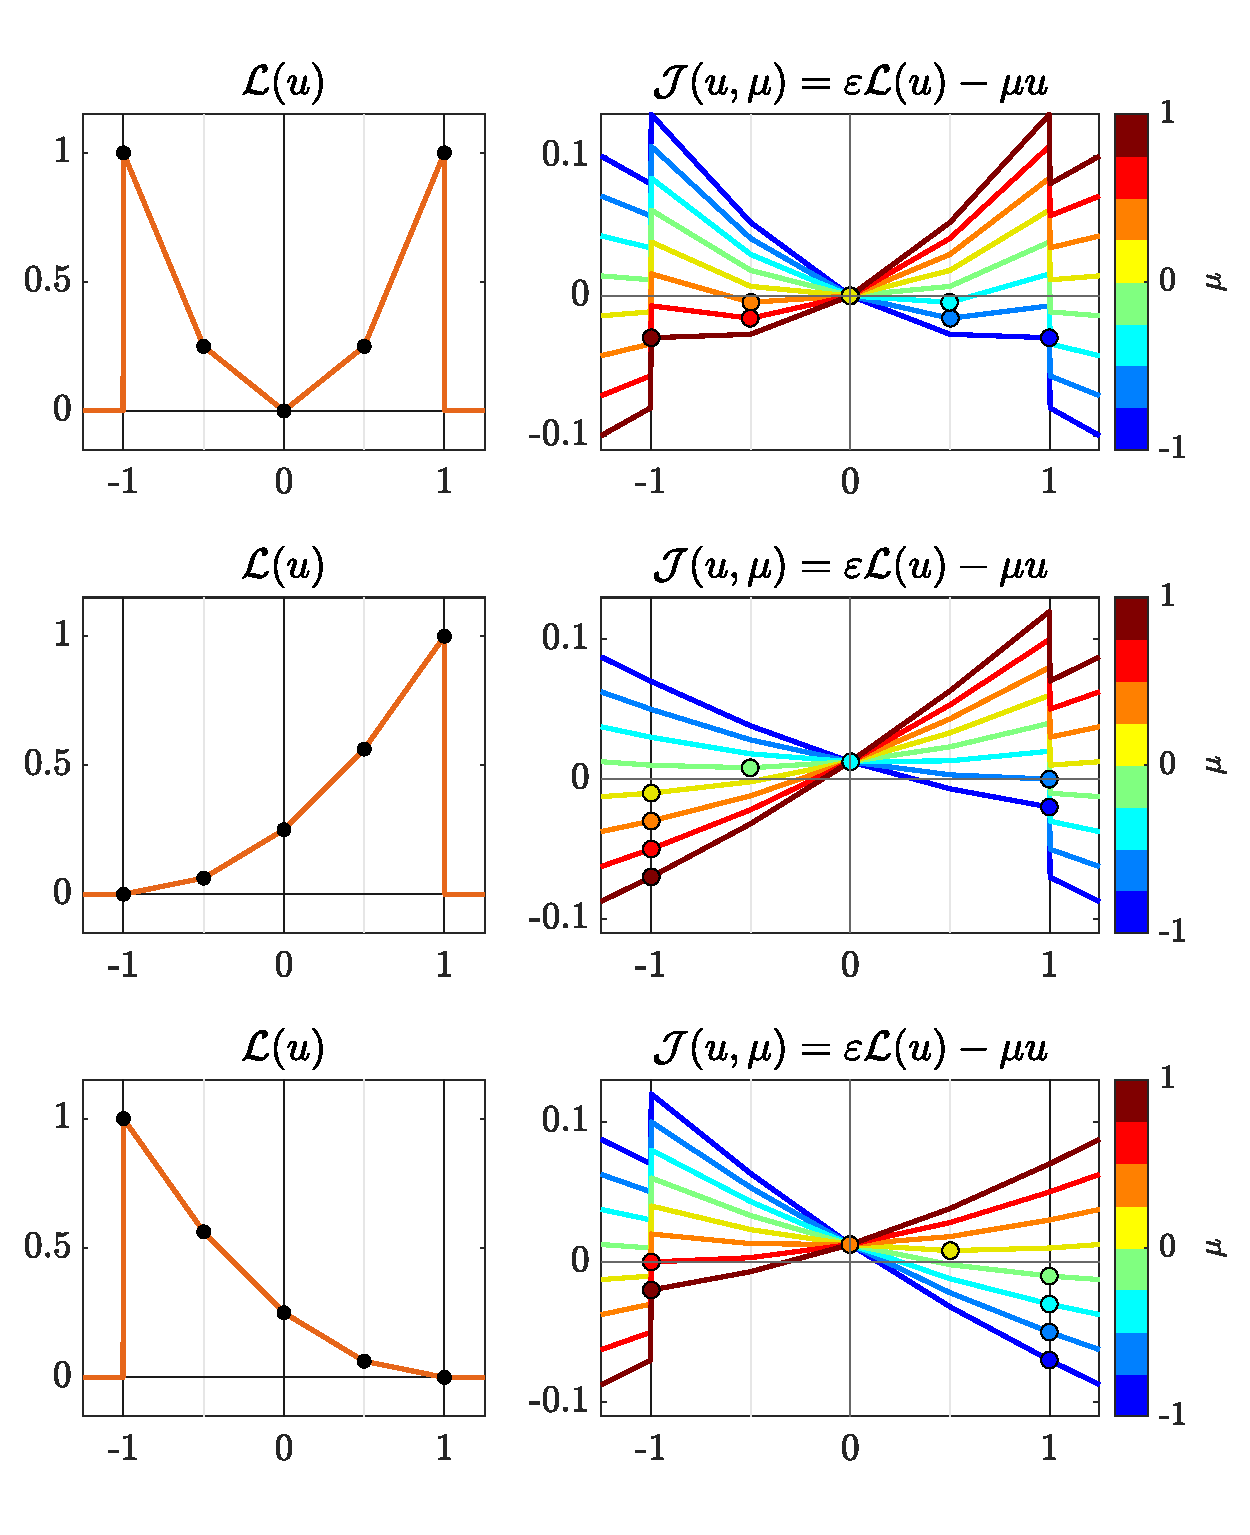
\includegraphics[scale=0.415]{img/fig04.eps}
    \caption{SHE Multi-nivel.} \footnotesize En la primera columna mostramos tres tipos de penalización concavas compatibles con la Proposición \ref{th:bang-bang}. A la derecha de cada una de ellas mostramos el comportamiento del Hamiltoniano para cada distintos valores de $m$ (colores). 
    \label{fig:SHE-multi}
\end{figure} 